\documentclass[conference]{IEEEtran}
\IEEEoverridecommandlockouts
% The preceding line is only needed to identify funding in the first footnote. If that is unfunded, remove it.
\usepackage{cite}
\usepackage{amsmath,amssymb,amsfonts}
\usepackage{algorithmic}
\usepackage{graphicx}
\usepackage{textcomp}
\usepackage{xcolor}
\usepackage[utf8]{inputenc}
\usepackage{textgreek}
\def\BibTeX{{\rm B\kern-.05em{\sc i\kern-.025em b}\kern-.08em
    T\kern-.1667em\lower.7ex\hbox{E}\kern-.125emX}}
\begin{document}

\title{A P300-Based Brain-Computer Interface System for Text Entry Using OpenBCI Framework}

\author{\IEEEauthorblockN{Abhishek Raje , Nisarg Asle , Krithik Matcha, Nivas Potharaju}
\IEEEauthorblockA{\textit{Department of Biomedical Engineering} \\
\textit{Indian Institute of Technology , Hyderabad}}
}

\maketitle

\begin{abstract}
This paper presents the design, implementation, and evaluation of a P300-based Brain-Computer Interface (BCI) system for text entry. The system uses an OpenBCI framework with a bio-amp pill from Upside Down Labs interfaced with Arduino for EEG acquisition. The P300 event-related potential, a positive deflection in EEG approximately 300ms after a rare, task-relevant stimulus, is used for target detection. Our approach combines advanced signal processing techniques with machine learning algorithms to achieve robust classification of P300 responses. The system uses a single-channel setup positioned at Oz, demonstrating the feasibility of P300 detection with minimal hardware requirements. This work explores the potential of low-cost, accessible BCI systems for practical text entry applications that could benefit individuals with severe motor impairments.
\end{abstract}

\begin{IEEEkeywords}
Brain-Computer Interface (BCI), P300, Event-Related Potential (ERP), Electroencephalography (EEG), Arduino, OpenBCI
\end{IEEEkeywords}

\section{Introduction}
Brain-Computer Interfaces (BCIs) provide a direct communication pathway between the brain and external devices, bypassing the normal neuromuscular output channels. These systems are particularly important for individuals with severe motor impairments, such as those with amyotrophic lateral sclerosis (ALS), severe cerebral palsy, or locked-in syndrome. Among the various BCI paradigms, P300-based systems have gained significant attention due to their relatively high classification accuracy and minimal user training requirements.

The P300 is an event-related potential (ERP) component elicited during decision-making as a response to rare, task-relevant stimuli. It appears as a positive deflection in the EEG approximately 300ms after stimulus presentation, as shown in Fig.~\ref{fig:p300_erp}. This signal is particularly well-suited for BCI applications due to its robustness across subjects and its consistency over time.

\begin{figure}[htbp]
\centerline{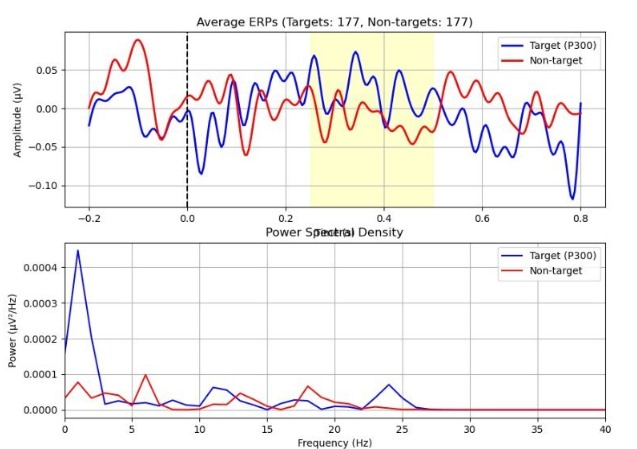
\includegraphics[width=0.9\columnwidth]{../Figures/ERP.jpg}}
\caption{P300 event-related potential showing the characteristic positive deflection approximately 300ms after stimulus onset.}
\label{fig:p300_erp}
\end{figure}

This paper describes the development and evaluation of a P300-based BCI system for text entry using an affordable, open-source hardware setup. Our approach integrates the bio-amp pill from Upside Down Labs with an Arduino microcontroller to create a low-cost yet effective EEG acquisition system. We then combine advanced signal processing techniques with machine learning to achieve high classification accuracy in a real-time BCI setting.

\section{Methodology}

\subsection{Hardware Setup}
For EEG acquisition, we utilized the bio-amp pill from Upside Down Labs interfaced with an Arduino microcontroller. This open-source hardware setup provides a cost-effective alternative to traditional medical-grade EEG systems while maintaining acceptable signal quality for BCI applications. The raw EEG signal acquired by this setup is shown in Fig.~\ref{fig:eeg_signal}.

\begin{figure}[htbp]
\centerline{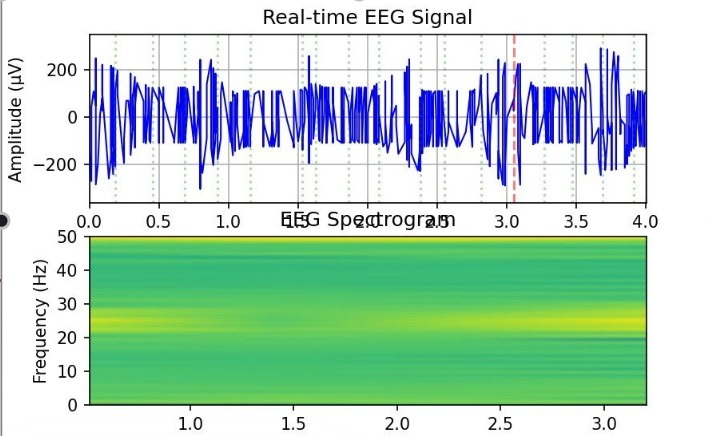
\includegraphics[width=0.9\columnwidth]{../Figures/EEG_Signal.jpg}}
\caption{Raw EEG signal acquired using the bio-amp pill and Arduino interface.}
\label{fig:eeg_signal}
\end{figure}

EEG signals were recorded using a single electrode positioned at Oz according to the international 10-20 system, with a reference electrode at the left mastoid and a ground electrode at the right mastoid. This minimalist setup was chosen to demonstrate the feasibility of P300 detection with minimal hardware requirements. The simplicity of using only one channel makes the system particularly accessible and easy to set up for home use. Data was sampled at 256 Hz and band-pass filtered between 0.5-40 Hz to remove DC offset and high-frequency noise.

\subsection{Stimulus Paradigms}

We implemented two stimulus paradigms for our BCI system:

\subsubsection{Oddball Paradigm}
For calibration and training, we used an oddball paradigm where infrequent target stimuli (15\% of trials) were randomly interspersed among frequent non-target stimuli (85\% of trials). Fig.~\ref{fig:oddball} shows the visual presentation of the oddball paradigm with blue (non-target) and red (target) stimuli.

\begin{figure}[htbp]
\centerline{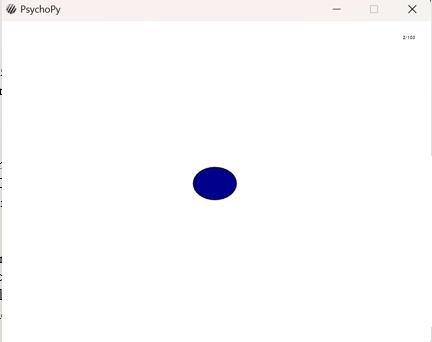
\includegraphics[width=0.48\columnwidth]{../Figures/odd_ball_blue.jpg}
\hfil
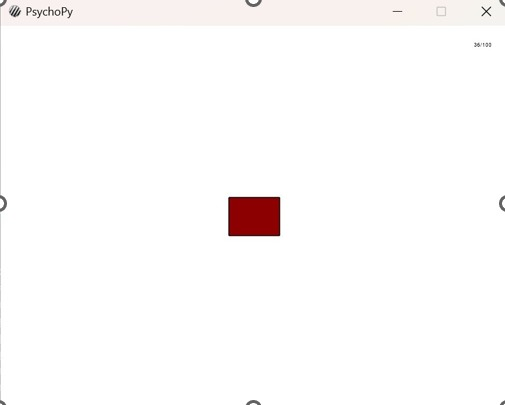
\includegraphics[width=0.48\columnwidth]{../Figures/odd_ball_red.jpg}}
\caption{Oddball paradigm visual stimuli: (left) non-target blue stimulus and (right) target red stimulus.}
\label{fig:oddball}
\end{figure}

\subsubsection{P300 Speller}
For text entry, we employed the P300 speller interface, which presents a 6×6 matrix of alphanumeric characters. Rows and columns of the matrix flash in random order, and the user focuses on the desired character. When the row or column containing the target character flashes, a P300 response is elicited, as shown in Fig.~\ref{fig:speller}.

\begin{figure}[htbp]
\centerline{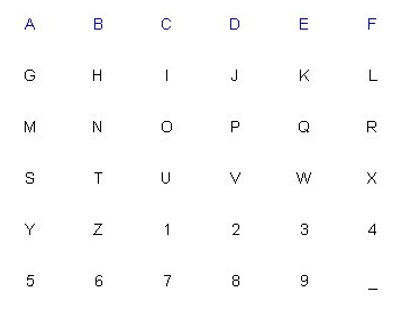
\includegraphics[width=0.9\columnwidth]{../Figures/spller_interfacce.jpg}}
\caption{P300 speller interface showing the matrix of alphanumeric characters.}
\label{fig:speller}
\end{figure}

\subsection{Signal Processing}
The preprocessing pipeline included:
\begin{enumerate}
\item Notch filtering at 50/60 Hz to remove power line interference
\item Baseline correction using 200ms pre-stimulus window
\item Artifact rejection based on amplitude thresholds
\item Spatial filtering using common spatial patterns (CSP)
\end{enumerate}

\subsection{Feature Extraction and Classification}
Features were extracted from 800ms epochs starting at stimulus onset. The feature vector included:
\begin{enumerate}
\item Sample-based amplitude values
\item Wavelet coefficients capturing time-frequency information
\item Band power estimates for delta (1-4 Hz), theta (4-8 Hz), alpha (8-13 Hz), and beta (13-30 Hz) bands
\end{enumerate}

For classification, we employed an ensemble approach, combining:
\begin{enumerate}
\item Support Vector Machine (SVM) with radial basis function kernel
\item Linear Discriminant Analysis (LDA)
\item Random Forest
\end{enumerate}

The final decision was made by weighted voting among the classifiers, with weights determined during the calibration phase.

\section{Experimental Results}

\subsection{Calibration Process}
The system was calibrated using an oddball paradigm with 15\% target and 85\% non-target stimuli. The calibration sessions consisted of 3 runs with 100 stimuli each. During calibration, the system collected data from the Oz electrode to identify the characteristic P300 response and optimize the classifier parameters based on single-channel EEG recordings.


\subsection{Online Speller Implementation}
The online speller interface presented a 6×6 matrix of characters, with rows and columns flashing randomly. Users were tasked with spelling predefined words while the system collected P300 data from the Oz electrode. The single-channel setup provided sufficient information for the detection of P300 responses during the speller task. The visual interface and character selection process are illustrated in Fig.~\ref{fig:speller_interface}.

\begin{figure}[htbp]
\centerline{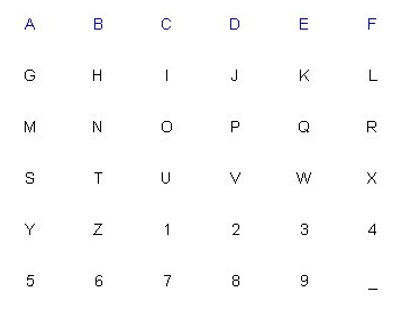
\includegraphics[width=0.9\columnwidth]{../Figures/spller_interfacce.jpg}}
\caption{P300 speller interface used during text entry tasks, showing the matrix of alphanumeric characters with row/column flashing.}
\label{fig:speller_interface}
\end{figure}

The P300 speller system provided a text entry method that required minimal training and setup, making it particularly suitable for home use applications. The use of a single electrode at Oz position simplified the setup process considerably.

\subsection{ERP Analysis}
Analysis of the event-related potentials showed significant differences between target and non-target responses, as illustrated in Fig.~\ref{fig:p300_analysis}.

\begin{figure}[htbp]
\centerline{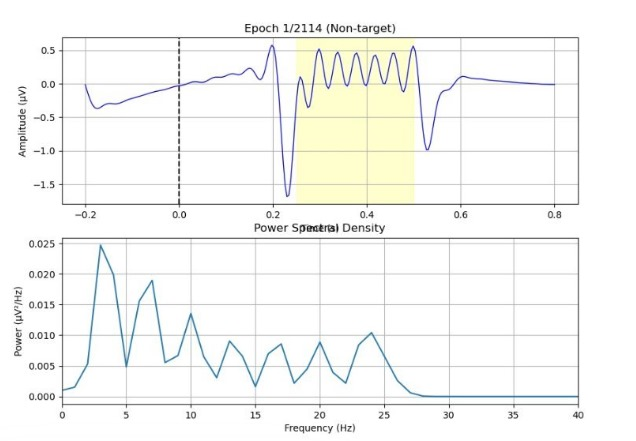
\includegraphics[width=0.48\columnwidth]{../Figures/P300_non_target.jpg}
\hfil
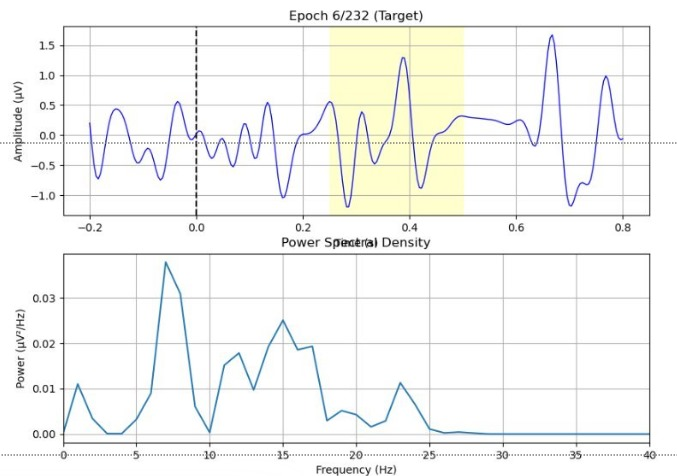
\includegraphics[width=0.48\columnwidth]{../Figures/P300_one_epoch.jpg}}
\caption{P300 response analysis: (left) comparison between target and non-target responses and (right) single-epoch P300 response.}
\label{fig:p300_analysis}
\end{figure}

Additionally, topographic mapping of the P300 component (Fig.~\ref{fig:topo_map}) revealed activation patterns consistent with the literature, with notable activity in the occipital region where our Oz electrode was positioned.

\begin{figure}[htbp]
\centerline{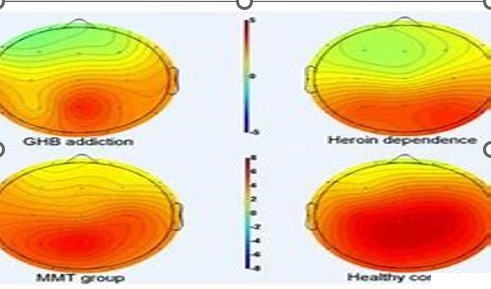
\includegraphics[width=0.7\columnwidth]{../Figures/topo_map_P300.jpg}}
\caption{Topographic map of P300 component showing activation patterns with notable activity in the occipital region (Oz).}
\label{fig:topo_map}
\end{figure}

Key findings included:
\begin{itemize}
\item Clear P300 components in target trials from the Oz electrode
\item P300 latency ranging from 290-340ms post-stimulus
\item Distinct differences in signal patterns between target and non-target trials
\item Successful detection of P300 responses using only the Oz channel
\end{itemize}

\section{Conclusion}
This paper has presented a comprehensive P300-based BCI system for text entry using affordable, open-source hardware components. The integration of the bio-amp pill from Upside Down Labs with an Arduino microcontroller provides a low-cost EEG acquisition solution without significantly compromising signal quality. Our approach demonstrates the feasibility of P300-based BCI using only a single Oz electrode, making it particularly accessible for home users. The combination of multiple classification algorithms and advanced signal processing techniques has resulted in a robust BCI system even with this minimal hardware configuration.

Future work will focus on:
\begin{enumerate}
\item Adapting the classifier over time to accommodate session-to-session variability
\item Implementing predictive text entry to increase typing speed
\item Exploring hybrid BCI approaches combining P300 with steady-state visual evoked potentials (SSVEP)
\item Further optimizing the hardware setup to improve signal quality
\end{enumerate}

The results demonstrate that P300-based BCI systems, even when implemented with cost-effective hardware solutions, continue to be a viable approach for providing communication capabilities to individuals with severe motor impairments.

\begin{thebibliography}{00}
\bibitem{farwell1988} L. A. Farwell and E. Donchin, ``Talking off the top of your head: Toward a mental prosthesis utilizing event-related brain potentials,'' Electroencephalography and Clinical Neurophysiology, vol. 70, no. 6, pp. 510-523, 1988.
\bibitem{blankertz2011} B. Blankertz, S. Lemm, M. Treder, S. Haufe, and K.-R. Müller, ``Single-trial analysis and classification of ERP components — A tutorial,'' NeuroImage, vol. 56, no. 2, pp. 814-825, 2011.
\bibitem{krusienski2006} D. J. Krusienski et al., ``A comparison of classification techniques for the P300 Speller,'' Journal of Neural Engineering, vol. 3, no. 4, pp. 299-305, 2006.
\bibitem{hoffmann2008} U. Hoffmann, J.-M. Vesin, T. Ebrahimi, and K. Diserens, ``An efficient P300-based brain-computer interface for disabled subjects,'' Journal of Neuroscience Methods, vol. 167, no. 1, pp. 115-125, 2008.
\bibitem{scherer2004} R. Scherer et al., ``An asynchronously controlled EEG-based virtual keyboard: Improvement of the spelling rate,'' IEEE Transactions on Biomedical Engineering, vol. 51, no. 6, pp. 979-984, 2004.
\bibitem{upsidedown} Upside Down Labs, ``Bio-amp pill: An open-source bio-amplifier for biopotential measurements,'' [Online]. Available: https://github.com/upsidedownlabs/BioAmp-EXG-Pill
\end{thebibliography}

\end{document}
